\section{Architecture}
\label{sec:Architecture}
Regarding the design of \teledroid\ Application, there are three main components in the architecture, as in 
Figure~\ref{fig:architecture}. Initially, we implement a file browser activity as our main activity in \teledroid\ app. 
Users are able to view all of the files in the Android file system. In addition, the file browser can open 
audio, plain text, and image files. We've used this file browser for testing purpose. Next, a long running local 
service can be started from the menu on the file browser activity. The service will stay connected with the server even when 
\teledroid\ is no longer visible. This background service serves to monitoring, scanning, and 
sync files with remote server. Finally, note that two sorts of threads are invoked by the background service. 
There's the \verb+FileMonitorThread+, and the \verb+ScanFilesThread+. We prefer to implement threads rather than all the
functions within one process because this enables us to decouple functionality and also make blocking calls.

\onecolumn
\begin{figure}[htp]
\centering
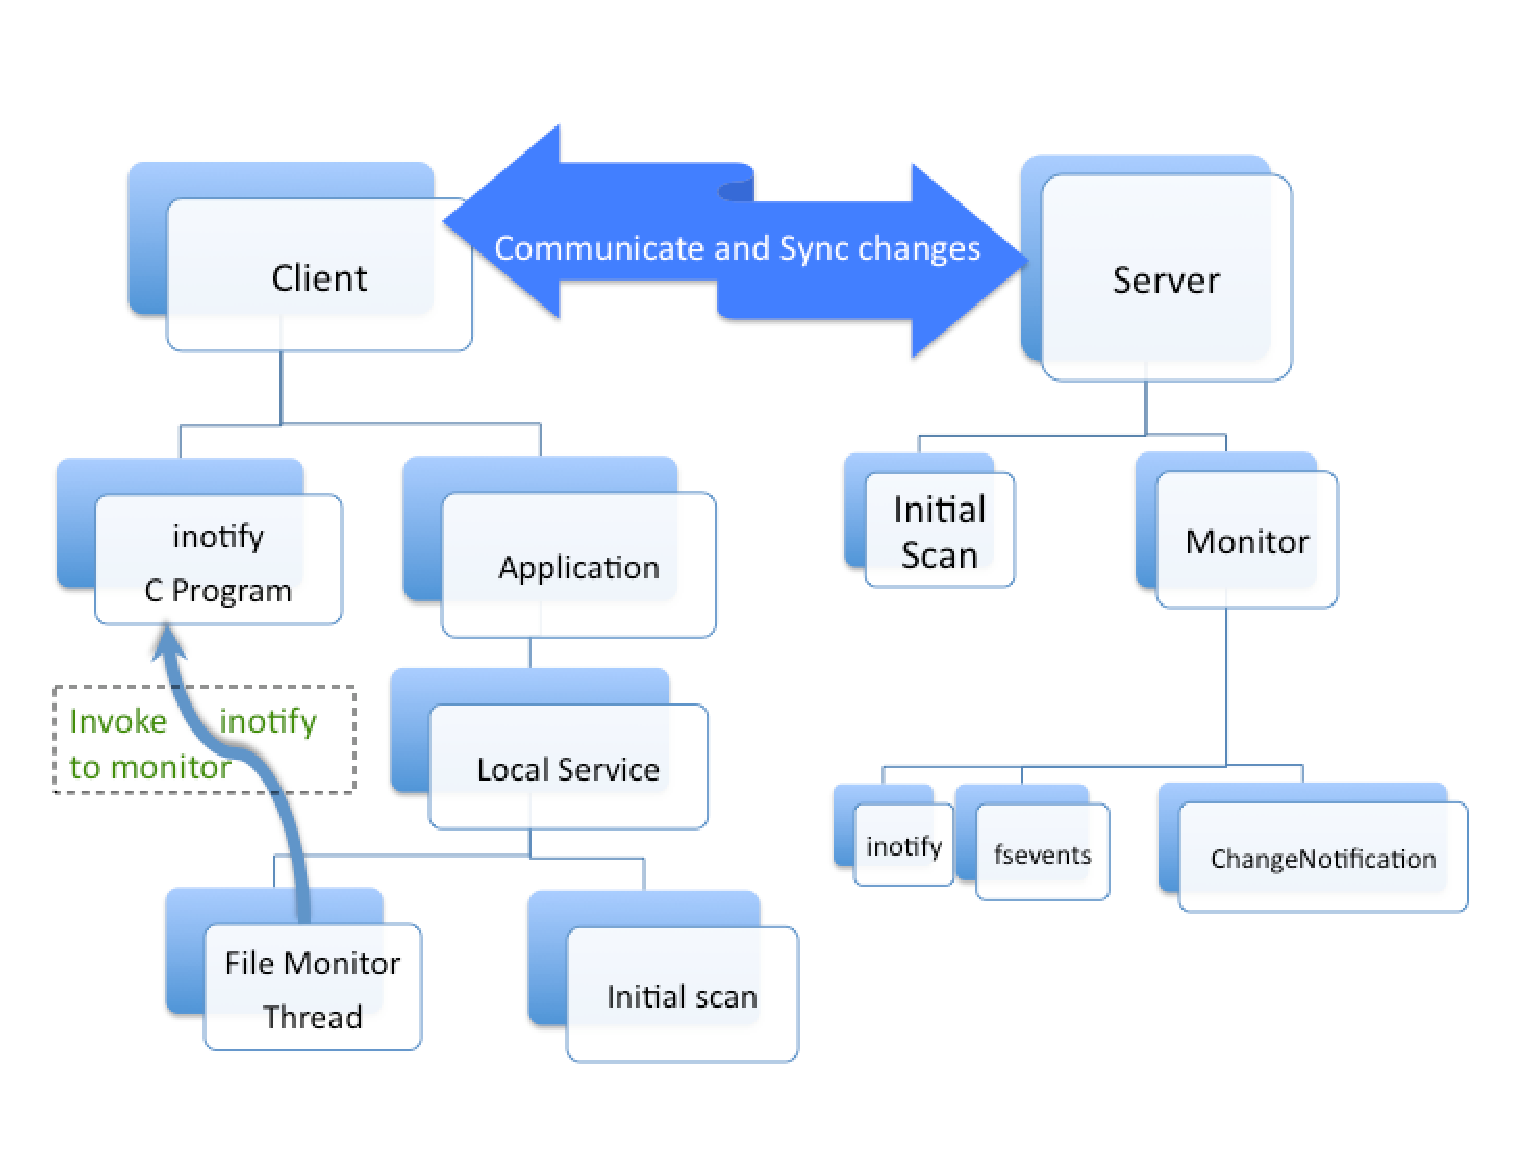
\includegraphics[scale=0.5]{architecture}
\caption{\teledroid\ Architecture}\label{fig:architecture}
\end{figure}
\twocolumn

\section{Implementation}
\label{sec:Implementation}
\subsection{Client Server Communication}
Our implementation of client-server communication and file transfer are based on JSch. JSch is a pure Java open source SSH library. We establish a connection with the remote server when the \teledroid application starts, and we keep the connection open, as our background service will communicate with remote server from time to time, and transfer files back and forth. 

The JSch library provides the ability to open different channels simultaneously using only a single connection, so that we avoid 
wasting time and resources establishing new connections. We implement a class \verb+Connection+ and use it as an abstraction over this interface, enabling us to open shell channels and transfer files over SCP. We implemented functions to open 
a shell for executing commands on the server side.  
We also implemented two functions: \verb+SCPTo()+ and \verb+SCPFrom()+ which follow the SCP protocol for transferring files, with some modifications to keep the modified times synchronized between client and server. 

We use simple depth-first walk of the given directory either when looking for changes in scan mode or registering files in monitor mode. When scanning we produce a mapping from filenames, relative to the initial directory that we're watching, to ModificationInfo objects, which store the modification time and other information necessary for determining how to synchronize.

By executing commands on the server, we can get a corresponding map from the server or register a directory to be monitored  and retrieve file change mappings. \teledroid\ will then compare the two mappings. If the difference of the modified time of the same file is bigger than a tolerance value (one second worked for our testing), then the younger copy of the file will be synced and replace the older one on the other side, while changing the modified time to be the same as the younger one. By this method, we are able to avoid the issue of syncing a file back and forth because the modified time of the file after replacement is newer than its source. More details on this can be seen below in the Synchronization section.

\subsection{File Change Notification}
Our application design requires a file change notification system, which should allow applications to request 
the monitoring of a set of files against a list of events. As the nature of running on mobile device, it should 
require as little system resources as possible and be easy to invoke in user space. 

Our implementation of filesystem monitors on the client is based on inotify. inotify is an inode-based file notification system 
that does not require a file ever be opened in order to watch it. It is designed with an interface that user space 
application could easily accessed through system calls. Also, inotify communicates with applications via a single 
file descriptor instead of signals providing simple and fast invocation.

For Linux, inotify was included in the mainline kernel from release 2.6.13 (June 18, 2005)\cite{Love:2005p1294}. We 
checked the default compilation options for Android and support for inotify was not removed. So we wrote a 
C program to make sure inotify worked in the emulator. The result was very encouraging. And we also found that in Android, 
the toolbox implements a simple notify program using inofity system calls. However, attempting to use the 
system provided notify program was unsuccessful. When the notify program was running, our program could inexplicably get nothing back from 
its stdout. After excluding the possibility of permission issues, we located the problem. The Android notify program will 
not flush its output stream after writing the result, so our application will block perpetually when reading from notify output stream. 

In our first release, we implement our own notify program, cross-compiled and pushed into the Android environment. This 
program simply implements the functionality of the original google notify program but flushes its output 
stream every time it finishes writing. The problem with this implementation is obvious. We have to create an extra process 
and stream with it to communicate. Also, in this system we cannot register and unregister files freely. 
We could only monitor a directory at a time, or we have to create multiple processes of the notify program, which will surely 
affect performance. 

In our release presented here, we use the Android JNI Library to invoke the inotify system calls. JNI is not officially supported by 
google, so there's no documentation for it. We implement a static class Notify as the interface to our notify library. 
In \verb+libnotify+, we use \verb+initNotify()+ to initialize inotify and get the file descriptor. We implement two 
methods: \verb+registerFile()+ and \verb+unregisterFile()+ for registering and releasing files to be monitored. 
We also implement \verb+hasNext()+, \verb+nextEvent()+ and \verb+eventMask()+ to get event information. And if the 
event is with a subfile of directory, we use \verb+newFile()+ to get sub file information. We cross-compiled the 
library and put the generated \verb+libnotify.so+ file into the lib directory for our application: 
\verb+data/data/net.solarvistas.android/lib/+, so that in the java static class Notify constructor, we could use 
\verb+System.loadLibrary(``notify'')+ to load the library. 

We met with a problem when compile the C library however, the JavaVM passed into \verb+JNI_Onload()+ cannot be correctly recognized 
as a struct. So we ignore the JNI\_VERSION check and implement a native method \verb+registerNativeMethod()+ to register 
the JNI native methods. We also include \verb+<utils/Log.h>+ so that we can log using the standard Android tools from within our JNI native code.

\subsection{Server Side Script}
The server-side portion of the project was broken into two parts, corresponding to the two phases of interaction with the server. Initially we construct a mapping of filename to modified time for each file in the portion of the filesystem we're synchronizing by doing a simple walk. This is inefficient in both time and space, but unavoidable, as monitoring for changes on both server and client side is only useful if they're initially synchronized.

After the client receives and processes the mapping of the entire directory, it launches a process that watches for changes. Two approaches were implemented here, pull and push. The pull-sync program gathers changes silently, sending them all in a batch on demand, while push-sync sends each change immediately, as it happens.

This work was implemented in the Factor programming language.  Factor is a high level, stack based language with an efficient optimizing compiler.  While a very interesting language in its own right, it is still a young language.  It was chosen for \teledroid purely for pragmatic reasons, however.  Due in part to its excellent foreign function interface, it is the only known environment with a cross-platform API for filesystem monitoring, with bindings for Linux's inotify, Mac OSX's fsevents, and a family of functions in the win32 API.

JSON was used as a serialization format as its impedance mismatch to our data – mostly maps from strings to long integers – was minimal.  JSON also had the advantage of actually being easy for humans to read while debugging.

The source of the server-side software is available separately at http://github.com/rictic/sync-monitor/tree/master

\subsection{Synchronization}
Synchronization is one of trickier elements in a distributed system. The issue in our \teledroid\ application is that the file after replacement will generate a new modified time, which is the current time and later than the file on the other side. Thus, the file on the other side will be replaced and also generate a newer modified time. Again and again, that file will be transferred back and forth even without any content modification. This is the result of applying the modified time as a key to the file comparison. We could employ checksums in our system, and this might relieve the issue, but with large files the performance impact could be undesirable. Our solution so far is that the new generated file will not be given the current time as its the modified time. Instead, it will be assigned with the modified time of that file on the other side. In this way, \teledroid\ is prevented from transferring files back and forth.

\subsection{Extra Parts}
(Riku)
